\chapter{Evaluation}
\label{evaluation}

This section is devoted to the description and discussion of three separate user
studies with the devices discussed in Chapter 2. Two studies were performed with
the original UCube device (one more informal than the other), while a longer
study involved both the SnapCAD and PopCAD systems.

\section{UCube Pilot}
\subsection{Procedure}
Early in 2011, we conducted an initial (and informal) pilot test of the UCube
with a group of 12-14 year olds. Fourteen participants, consisting of five girls
and nine boys, were divided into six groups (five groups of two, one group of
four). Participants were asked to model a sequence of five shapes of increasing
complexity using the UCube along with the companion software. The target shapes
were displayed on one half of a computer screen, while the UCube software
showing the live model was displayed on the other half as in
\autoref{fig:ucube_test1}.
The first shape that participants were asked to model was a straight vertical
line; after this, the requested shapes were a diagonal line, a cube, a
triangular prism, and finally an irregular polyhedral object. No shape required
more than four towers to complete, and shapes were always presented in the same
order.

\begin{figure}[h]
\begin{center}$
\begin{array}{cc}
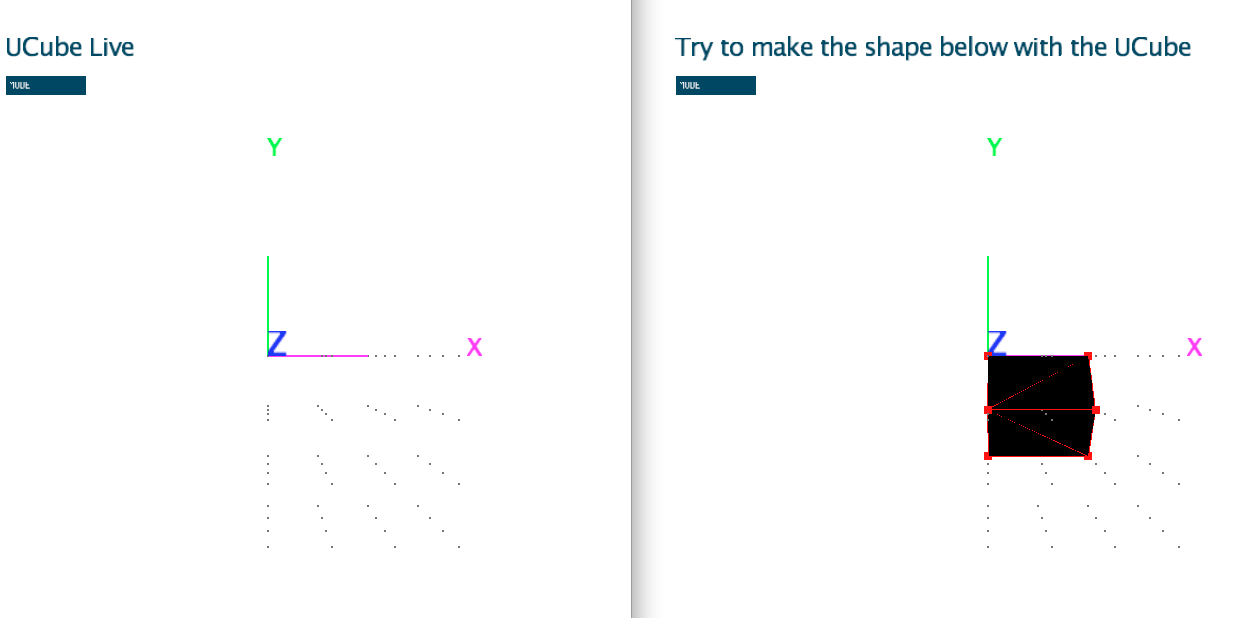
\includegraphics[width=.8\linewidth]{images/ucubescreentest}
\end{array}$
\end{center}
\caption{A screenshot of the testing setup, with the live output from the UCube
on the right and the target shape on the left.}
\label{fig:ucube_test1}
\end{figure}

Participants were instructed to place the poles on the board (but not shown
how), and were told that the software model could be rotated and filled in using
the keyboard and mouse, should that help them complete the task. The
participants were not given any hints as to how to complete the shapes and were
not told when they had the correct configuration (they had to indicate their
belief that the model was done). Participants were also instructed to 'think
aloud' about their actions. The main purpose of the pilot study was to get an
initial impression of how the UCube would act as an accessible 3D modeling
tool�how well it could help ``3D novices'' overcome the ``2D bottleneck''.

\subsection{Results and Discussion} 
Of the six groups who participated, four groups successfully modeled all five
shapes, one group ran out of time after three shapes, and one group finished one
shape. Sessions lasted between 17 and 30 minutes.
A variety of problem-solving strategies were observed during testing, as the
participants tended to treat the exercise as a sort of puzzle to be solved.
Simple methods equivalent to ``try and see'' were common, and seemed to serve as
a base point from which to draw conclusions about the relationship between the
3D model and 2D on-screen representation (e.g. ``No, not there, up one''). More
sophisticated strategies were also observed� ``deconstructing'' more complex
shapes into smaller, easier-to- model shapes (e.g. thinking of one side of a
cube as a square) was observed from several groups. Another popular technique
was to systematically match the on-screen perspective from the live model with
the shape they were attempting to model (e.g. ``Okay, first let's do the top
view, and then go from the side''). By orienting the two models similarly,
participants were able to make more accurate modeling decisions as well as check
their model against the on-screen shape. Counting distance in terms of spaces on
the board, between switches, or between dots on the screen was also a very
common technique of reasoning about and describing position. For example, by
counting that two vertices of a shape were separated by ``two dots over and one
down'' on the screen, subjects were able to count the distance out on the
physical UCube board. A few of the more mathematically-advanced participants
used terms such as ``axis'' and ``origin'' to orient themselves and describe
various positions on the board to their partners.
Another revealing observation in the pilot study was that, in the few instances
of mechanical failure (certain switches not lighting up, towers not plugging in
properly, or points not showing up on screen) the participants were still able
(with a high degree of certainty) to complete the assigned tasks. This appears
to indicate that, as opposed to arbitrarily moving the towers around until the
two sides of the computer screen looked the same, participants had formed a more
substantial mental model of the relationship between the UCube interface and the
2D representations on the screen. That opens the possibility that by performing
the embodied interactions necessary to operate the UCube, participants had
actually strengthened their understanding of how 3-dimensional space is
typically represented on a 2D screen. Although further testing and observation
is needed, this finding would strengthen the argument for using the UCube in an
educational setting to improve understanding of 3D space, as well as providing a
gateway for youngsters to move on to more complex modeling software.
While the variety of problem-solving techniques we witnessed is a testament to
the participants' ingenuity, it is also indicative of the fact that parts of the
UCube are not immediately intuitive. While none of the participants had trouble
understanding how to place the towers on the platform, the positions of the
towers and switches had to be reasoned out explicitly. It was common for groups
to clear the board of any poles when starting a new shape, even in cases where
an overlap of points or tower positions existed. (Figure XXXX, for example�shown
earlier in the context of explaining the UCube's operation�depicts one of the
students placing a tower and checking the screen to see whether the tower
placement is appropriate.) Although most groups completed all the shapes (or ran
out of time), there were some expressions along the way of the difficulty of the
task (e.g. ``This is hard'', or ``This is like a puzzle''). This indicates that
design changes can be made in future iterations to help clarify the
correspondence between positions on the UCube platform and the on-screen
representation; for example, labeling the both the physical and software grid
with a simple alphanumeric system.
Despite these drawbacks as well as the inherent limitations of the UCube design,
these early results indicate a promising ability of youngsters to effectively
engage with the UCube interface. In fact, despite various levels of success in
completing the assigned tasks, the vast majority of participants exhibited a
high level of engagement with the UCube. For example, although the group that
completed only one shape seemed unmotivated to attempt to model the other
shapes, they continued to play with the interface and observe the results, even
stating ``this is fun'' and ``I like the switches''. Participants also saw
potential uses for the UCube outside of the specific exercise we assigned.
Comments (unsolicited) included, ``you should use this to teach geometry'' and
``you could make this a puzzle game''.
At the very least, these early results indicate that the majority of
participants were able to take a 2-dimensional representation on the screen and
model its 3-dimensional equivalent using the UCube, a very encouraging result in
our eyes.

\section{Further UCube Study}

Early in 2012, we conducted a further user study of the UCube with a group of
11-13 year olds. The group consisted of ten participants, eight boys and two
girls, from a local middle school multimedia class. Every participant was
individually led through two separate exercises (outlined below) using the
UCube. 

\subsection{Procedure: Modeling}
Participants were handed a 3D-printed shape (modeled and printed from the UCube)
and were instructed to attempt to model the shape using the UCube. The
participant was initially allowed to hold the shape for approximately 10
seconds, after which they would hand the shape back to the facilitator and
attempt to model the shape from memory. Participants were instructed that they
may ask to hold the shape again, at which point they were allowed to hold it
throughout the duration of the modeling task. Additionally, users were
instructed that they had the option to skip a shape and return to it at a later
point in the exercise.
The five physical shapes presented were: a cube, a tetrahedron, a diamond, a
``house'' (a cube with a pyramid on top), and a complex irregular polyhedron.
The models were presented to the user starting with the cube (as this was deemed
to be the most basic shape with regard to modeling complexity). To avoid an
ordering bias, we randomized the presentation sequence of the next four shapes
using an online random order generator. If, after skipping a shape and returning
to it, the participant was still having difficulty, we offered them the
opportunity to attempt modeling the shape with the help of the UCube software,
the effects of which are discussed in the results section. Participants were
given a total of 25 minutes for the modeling exercise. We recorded, but did not
limit the modeling time per shape, only the total time for all five shapes.

\subsection{Procedure: Matching}
Participants were instructed to face away from the UCube while the facilitator
modeled a set of lights on the UCube corresponding to one shape among a set of
physical models laid out on the table next to the UCube.
Once the lights on the UCube were set up, the participant was instructed to turn
around, and indicate which physical object they thought the set of lights on the
UCube corresponded to.
There were nine physical models presented on the table, and consisted of a cube,
a tetrahedron, the �house� shape, a diamond, a triangular prism, an elongated
hexagon, a parallelogram, a trapezoid, and an irregular polyhedron (see
\autoref{fig:ucube_shapes} for a picture of all the models). The shapes were
always presented on the table in the same order and orientation to avoid
discrepancies in perception or association.
Of the nine shapes, the participants were asked to match five of them (the cube,
the triangular prism, the parallelogram, the elongated hexagon, and the
trapezoid). Thus, only the cube was presented in both the matching and modeling
exercises. As with the modeling exercise, the cube was presented first, with the
remaining four shapes presented in a computer-generated randomized
order.Participants were given a total of ten minutes for the matching exercise,
corresponding to two minutes per shape, and were instructed to think aloud
during the process.

\begin{figure}[h]
\begin{center}$
\begin{array}{cc}
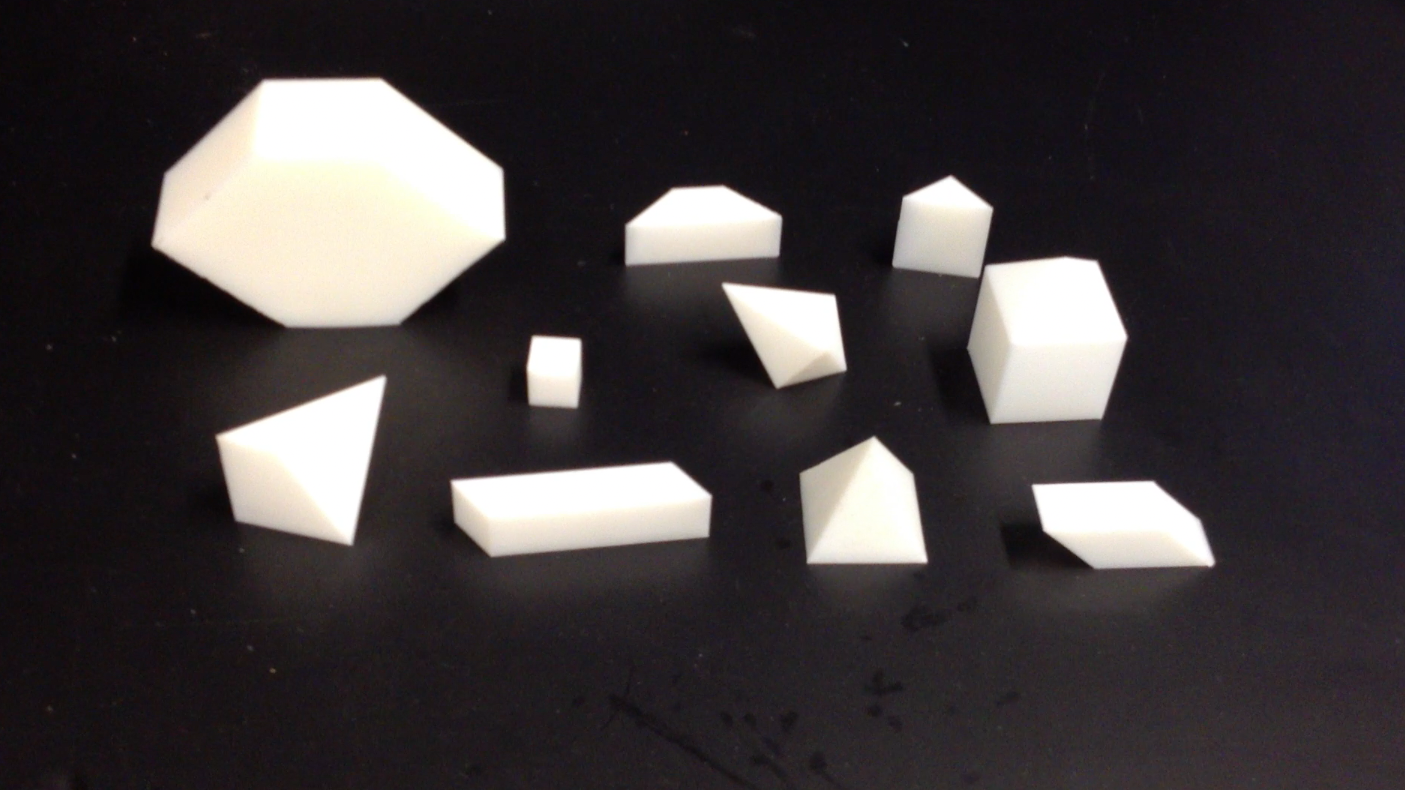
\includegraphics[width=.8\linewidth]{images/ucube_shapes}
\end{array}$
\end{center}
\caption{The nine 3D-printed models used in the modeling and matching tasks
described in this section.}
\label{fig:ucube_shapes}
\end{figure}


\subsection{Results} 
While many established forms of 3D modeling systems can be confounding and
operationally too complex for a child to navigate, the UCube was positively
received and system instruction was accomplished with just a minor introduction
and demonstration (system instruction and demonstration lasted approximately 2-3
minutes). We found this first instance of system comprehension to offer some
validation that the UCube worked well as a user-friendly 3D modeling device.
This section will detail the outcome of both the modeling and matching tasks
performed.

\subsubsection{Exercise 1: Modeling} 
Modeling occurred under three conditions:recreate the object from memory,
construction of the object while it was in the participant�s possession, and
modeling the shape with the help of the UCube software. Overall, 21 of 50 shapes
were completed from memory, 12 of 50 were completed while holding the shape, and a
further 8 of 50 were completed with the aid of the UCube software, for a total
of 41 out of 50 shapes modeled successfully (82\%). Of the nine missed shapes,
seven were of the same shape, the complex polyhedron. The remaining two misses
were from the same participant, who ran out of time before completion.
Of the 10 participants, 8 were able to recreate the cube from memory, whereas
only 4 were able to recreate the diamond and the tetrahedron from memory. Half
of the participants constructed the house from memory, and no participants were
able to complete the irregular polyhedron from memory. However, once shown the
software the majority of the participants found the modeling task significantly
easier to perform. The irregular polyhedron was by far the hardest shape and was
only able to be completed by 3 of the 10 participants either after continued
possession of the shape or using the software.

\begin{figure}[h]
\begin{center}$
\begin{array}{cc}
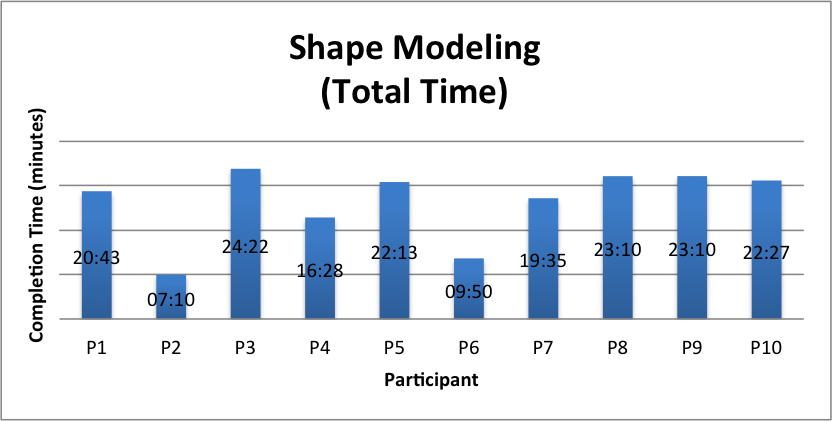
\includegraphics[width=.45\linewidth, height=1.75in]{images/modeling1}&
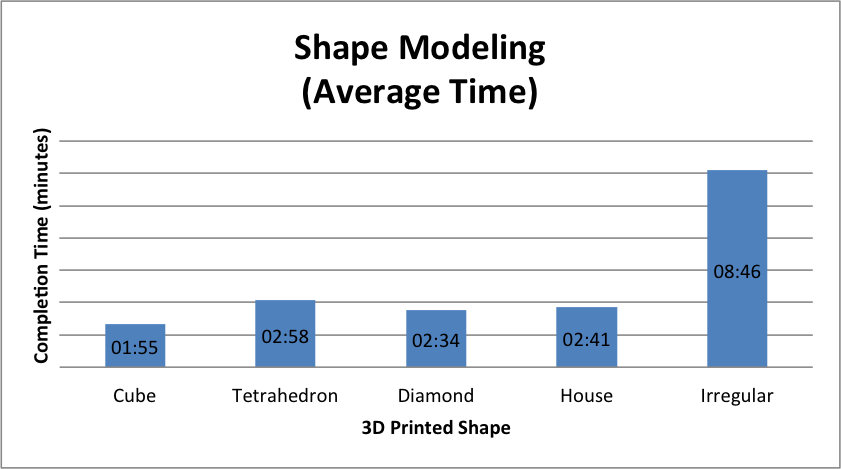
\includegraphics[width=.45\linewidth, height=1.75in]{images/modeling2}
\end{array}$
\end{center}
\caption{Results of the modeling task, showing total modeling time spent per
participant (left) and average modeling time spent per shape across
participants (right).}
\label{fig:modeling}
\end{figure}


\autoref{fig:modeling} represents the total completion times per participant (on
the left) and average time per shape (right). Two exceptional completion times
were observed, where participants finished modeling all the shapes in under 10
minutes. However, the majority of participants finished the task in the 19-25
minute range. Only one of the participants ran out of time. Once participants
had been introduced to the software, 9 of 10 of participants were able to
complete all but the irregular polyhedron. It is interesting to note that of the
10 participants, the child that had the most difficult time modeling, the lowest
shape completion rate, and the longest completion time during the matching
exercise was the youngest participant.


\subsubsection{Exercise 2: Matching} 
Out of 50 matching tasks (five per participant), all but three tasks were
completed in 20 seconds or less. \autoref{fig:matching} displays the total time
spent on the matching task per participant (left) and the average completion
times for each shape (right).
No participant selected the wrong shape (a few preliminary ``mis-selections''
were made that the participants quickly corrected), and all participants
completed the task in well under the allotted 10 minutes. The lack of errors in
the matching task is highly encouraging as a basis from which to reason about
youngsters' abilities to perceive and reason about convex hulls as a set of lit
vertices in space, meaning that this kind of 3D modeling interface might be
applied to other domains (e.g., as a cognitive assessment tool, a puzzle game,
etc.) with some optimism.

\begin{figure}[h]
\begin{center}$
\begin{array}{cc}
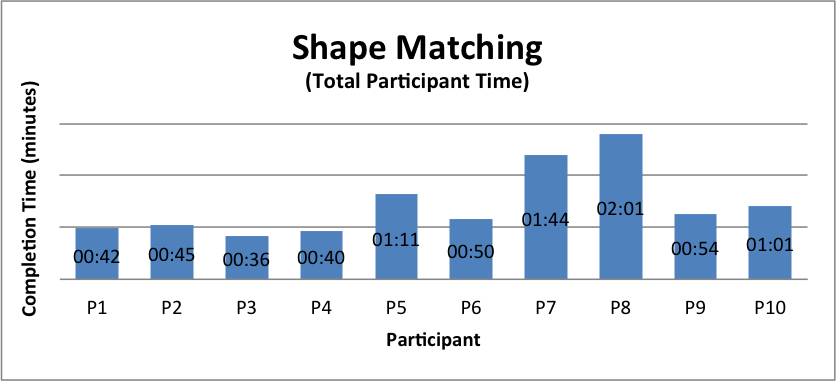
\includegraphics[width=.45\linewidth, height=1.75in]{images/matching1}&
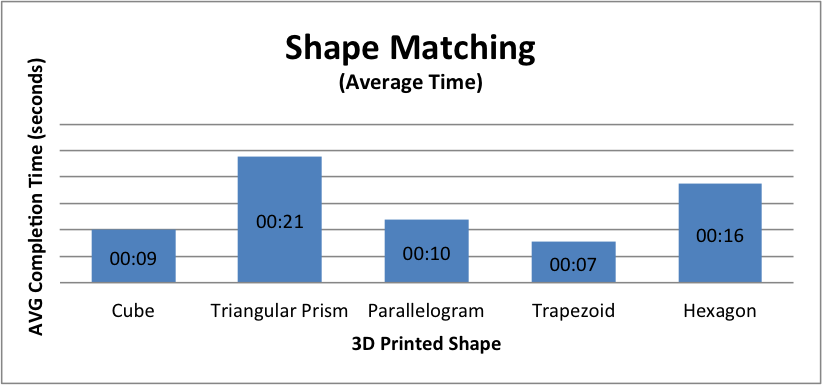
\includegraphics[width=.45\linewidth, height=1.75in]{images/matching2}
\end{array}$
\end{center}
\caption{Results of the matching task, showing total time spent per
participant (left) and average time spent per shape across
participants (right).}
\label{fig:matching}
\end{figure}


\subsubsection{Observations} 
Modeling trends as well as distinct modeling behaviors were documented in the
process. Common observations included building from the ground up (lowest
vertices first), building in the orientation that the object had been presented
in, not clearing the poles/lights from the UCube before starting to model a new
shape, and modeling a shape by breaking it up into discrete parts (e.g. a
participant building a house would commonly build a cube first and then add on a
vertex to the top; a participant constructing the diamond might combine two
opposite facing triangles.).

Unique behaviors were exhibited in the modeling process as well, reflecting a
type of user-specific construction-based problem- solving. One participant used
their arm to connect the red lights of the UCube for shape definition. A few
participants oriented the object differently than how it had been
presented�typically this occurred for the modeling of those objects with a
pyramidal apex (tetrahedron, house, diamond). Apex formation was perhaps one of
the most difficult concepts for most participants to grasp, as it required them
to strategically align the base on a 3x3 grid so there was a middle plug for
them to create the apex. If participants were fixated on designing from a 4x4
grid then there was no center plug for them to create a midpoint. Some
participants ended up building an oblong polyhedron as opposed to a cube, or an
oblique polyhedron as opposed to an equilateral tetrahedron. Other observed
behaviors included a participant who modeled shapes by turning on lights for an
entire shape edge, as opposed to just the corners and a participant who built
shapes that were floating, as opposed to resting on the base of the UCube.
There were also some notable behaviors regarding physical and gestural actions
of the participants. Many participants modeled with both hands simultaneously,
placing towers and flipping switches without a clear preference for a dominant
hand. Participants would often gesture with their arms following an arc in
parallel with a face of the object they were currently modeling. This �tracing�
behavior was also noticed when participants were holding a physical model and
tracing a side of the object with their fingertip, often while rotating the
object with the other hand. Finally, during object possession phase three
participants actually placed the 3D object on top of the UCube in the modeling
space while they reasoned out the construction (see
\autoref{fig:user_placedModel} for an example).

\begin{figure}[h]
\begin{center}$
\begin{array}{cc}
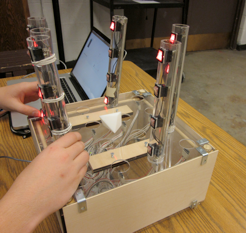
\includegraphics[width=.45\linewidth]{images/idc3}
\end{array}$
\end{center}
\caption{A participant modeling with the UCube, using a strategy of placing the
physical model on top of the UCube while modeling, as well as using both hands
simultaneously to manipulate the towers.}
\label{fig:user_placedModel}
\end{figure}



\section{SnapCAD and PopCAD}
The study will comprise several stages, the first being a pre-assessment of
spatial reasoning skills (all spatial reasoning assessment will be done using
the 'Children's Mental Transformation Task' designed by Susan Levine - see
http://silccenter.org/index.php/testsainstruments#MRT for the instruments, see
http://www.spatialintelligence.org/publications_pdfs/Ehrlich\%20Levine\%20\%20Goldin-Meadow\%20\%282006\%29.pdf
 p.1260-1261 for a good description of the study procedure.). After the
pre-assessment, participants will be split into two groups (~10 students each),
with group A modeling first on the PopCAD and group B modeling first on the
SnapCAD (a similar modeling device made from more rigid materials, and
representing a more expressive potential modeling space with a different means
of selecting points in space).
The evaluating of each device will consist of three modeling exercises,
evaluating the three main modeling modes in the software: convex hull, path, and
minimal spanning tree.  The basic operation and a brief explanation of each mode
will be given to the participants before each new modeling mode. Four 3D-printed
models representative of each mode will be presented to the user in a random
order, for a total of 12 modeling tasks. The random order shall be determined by
a computer program, and each task will be cut off at 10 minutes. Successful
completion (or lack thereof), time to completion, and observational notes shall
be recorded for each task. Participants will be asked to �think aloud� about
their process, difficulties, modeling choices, etc. Video will be recorded for
the purposes of analyzing user gestures when asked about how they arrived at a
certain solution.
A freehand activity will occur before and after the modeling tasks (10 minutes
each time) to help to get a sense of the kinds of shapes and modes used, the
overall usability of the interface, and a sense of the expressive range of the
relative point arrays, (PopCAD has a 3x3x3 equidistant grid of 27 individual
points, SnapCAD has a 7x7x7 grid of 343 points). By asking participants to think
aloud about their intentions and thinking processes, a deeper understanding may
be gained of the strengths and weaknesses of the system. Additionally, the
modeling modes used, relative time spent using each mode, and complexity (in
number of points) of the final object modeled will be recorded.
After the first set of modeling tasks, users will be given a mid-term assessment
using the same Mental Transformation Task as before (although different
individual problems will be presented). A week or so later, participants will
model on the device they have not used. Exercises will be consistent by device,
but may differ slightly between devices in order to tease out some of the
potential differences in each design. Once modeling on the second device is
completed, users will take final assessment to gauge if any improvement in
spatial reasoning skills has occurred throughout the study.
Around 20 participants will be enrolled in the study. Each individual session
should take 2 hours or less, and the overall duration of the study will be three
weeks. No control group will be used.

After the consent and assent forms are completed and the study session starts,
participants will be seated and will go through an explanation of the entire
study and what they will be asked to do. The pre-assessment will then be given,
consisting of 10 brief exercises where the participant attempts to match a
spatially transformed shape, printed on paper along with several incorrect
choices, to its original counterpart.

Participants will then be seated in front of a desk on which either the PopCAD
interface (a pop-up book) or SnapCAD (a tower and magnetic light based
interface) has been placed. The device will be hooked up to a laptop on the
desk. Participants will be given a brief demo of how to interact with the device
and how the software responds to those interactions.

The tasks that follow are the same for each device:

Task 1: Convex Hull Modeling

The participant will be given a brief demo of how the �convex hull� modeling
mode interprets the points from the device. The user will then be presented with
a series of four (4) plastic, 3D-printed models that were modeled on the device
using �convex hull� mode. The 4 shapes will be presented in a computer-generated
random order. For each of these shapes, the participant will attempt to recreate
the shape using the modeling abilities of the device. The user will be
instructed to indicate when they believe they are done, as well as to think
aloud about their modeling process. Each modeling task will be capped at 10
minutes. The time to completion (of lack thereof), observational notes, and
video shall be recorded.

Task 2: Path Modeling

The participant will be given a brief demo of how the �path� modeling mode
interprets the points from the device. The user will then be presented with a
series of four (4) plastic, 3D-printed models that were modeled on the device
using the �path� mode. The 4 shapes will be presented in a computer-generated
random order. For each of these shapes, the participant will attempt to recreate
the shape using the modeling abilities of the device. The user will be
instructed to indicate when they believe they are done, as well as to think
aloud about their modeling process. Each modeling task will be capped at 10
minutes. The time to completion (of lack thereof), observational notes, and
video shall be recorded.

Task 3: Minimal Spanning Tree Modeling

The participant will be given a brief demo of how the �minimal spanning tree�
(aka �tree�) modeling mode interprets the points from the device. The user will
then be presented with a series of four (4) plastic, 3D-printed models that were
modeled on the device using the �tree mode. The 4 shapes will be presented in a
computer-generated random order. For each of these shapes, the participant will
attempt to recreate the shape using the modeling abilities of the device. The
user will be instructed to indicate when they believe they are done, as well as
to think aloud about their modeling process. Each modeling task will be capped
at 10 minutes. The time to completion (of lack thereof), observational notes,
and video shall be recorded.

Task 4: Freehand Modeling

The freehand activity will occur before and after the modeling tasks and will
serve to get a sense of the overall usability of the interface as well as a
sense of the expressive range of each device. By asking participants to think
aloud about their intentions and thinking processes, a deeper understanding may
be gained of the strengths and weaknesses of the system. Additionally, the
modeling modes used, relative time spent using each mode, and complexity (in
number of points) of the objects modeled will be recorded.



